\documentclass[11pt]{beamer}
\usepackage{fontspec}
%\defaultfontfeatures{Mapping=tex-text}
\usefonttheme{serif}
\setbeamercolor{titlelike}{fg=blue}
\setbeamercolor*{author}{parent=title}
\setbeamercolor*{institute}{parent=title}
\setbeamercolor*{date}{parent=title}

\usepackage[utf8]{inputenc}
\usepackage{amsmath}
\usepackage{amsfonts}
\usepackage{amssymb}
\setbeamertemplate{footline}[frame number] % make page number
\setbeamertemplate{frametitle}[default][center] % make title and page title center
\author{Zepu Xi\\Followed Prof. Vladimir N. Vapnik}
\title{COMPLETE STATISTICAL THEORY OF LEARNING\\LEARNING USING STATISTICAL INVARIANTS}
\setbeamercovered{transparent} 
\setbeamertemplate{navigation symbols}{} 
%\logo{} 
\institute{Sun Yat-sen University} 
\date{\today} 
\subject{} 
\begin{document}

\begin{frame}
\titlepage
\end{frame}

%\begin{frame}
%\tableofcontents
%\end{frame}

\section{PART I: VC THEORY OF GENERALIZATION}
\begin{frame}
{\color{blue}{
\begin{center}
PART I
\end{center}
\begin{center}
VC THEORY OF GENERALIZATION
\end{center}
}}
\end{frame}


\begin{frame}{THE MAIN QUESTION OF LEARNING THEORY}
\begin{center}
QUESTION:

When in the set of functions $\{f(x)\}$ we can minimize functional
\begin{align*}
R(f) = \int L(y, f(x))dP(x,y), \quad f(x) \in \{f(x)\},
\end{align*}
if measure $P(x,y)$ is unknown but we are given $\ell$ iid pairs
\begin{align*}
(x_{1}, y_{1}), \ldots, (x_{\ell}, y_{\ell}).
\end{align*}

ANSWER:

We can minimize functional $R(f)$ using data \emph{if and only if} the VC-dimension $h$ of set $\{f(x)\}$ is finite. 
\end{center}
\end{frame}


\begin{frame}{DEFINITION OF VC DIMENSION}
Let $\{\theta(f(x))\}$ be a set of indicator functions \\(here $\theta(u) = 1$ if $u \geq 0$ and $\theta(u) = 0$ is $u < 0$).

\begin{enumerate}
\item[•] VC-dimension of set of indicator functions $\theta(f(x))$ is equal $h$ if $h$ is the maximal number of vectors $x_{1}, \ldots, x_{h}$ that can be shattered (separated into all $2^{h}$ possible subsets) using indicator functions from $\{\theta(f(x))\}$. If such vectors exist for any number $h$ the VC dimension of the set if infinite.
\item[•] VC-dimension of set of real valued functions $\{f(x)\}$ is the VC-dimension of the set of indicator functions $\{\theta(f(x)+b)\}$.
\end{enumerate}
\end{frame}

\begin{frame}{TWO THEOREMS OF VC THEORY}
\begin{theorem}
If set $\{f(x)\}$ has VC dimension $h$, then with probability $1-\eta$ for all functions $f(x)$ the bound
\begin{align*}
R(f) \leq R_{\text{emp}}^{\ell}(l) + \sqrt{e^{2} + 4eR_{\text{emp}}^{\ell}(f)},
\end{align*}
hold true, where
\begin{align*}
R_{\text{emp}}^{\ell} = \frac{1}{\ell}\sum_{i=1}^{\ell}L(y_{i}, f(x_{i})), e = O\left(\frac{h - \ln \eta}{\ell}\right).
\end{align*}
\end{theorem}


\begin{theorem}
Let $x, w \in R^{n}$. The VC dimension $h$ of set of linear indicator functions $\{\theta(x^{T}w): ||x||^{2} \leq 1, ||w||^{2} \leq C\}$ is 
\begin{align*}
h \leq \min(C, n) + 1.
\end{align*}
\end{theorem}
\end{frame}

\begin{frame}{STRUCTURAL RISK MINIMIZATION PRINCIPLE}
To find the desired approximation $f_{\ell}(x)$ in a set $\{f(x)\}$:
\begin{enumerate}
\item[FIRST] introduce a structure on a set of functions $\{f(x)\}$
\begin{align*}
\{f(x)\}_{1} \subset \{f(x)\}_{2} \subset \ldots \subset \{f(x)\}_{m} \subset \{f(x)\}
\end{align*} 
with corresponding VC-dimension $h_{k}$
\begin{align*}
h_{1} \leq h_{2} \leq \ldots \leq h_{m} \leq \infty.
\end{align*}
\item[SECOND] chose the function $f_{\ell}(x)$ that minimizes the bound
\begin{align*}
R(f) \leq R_{\text{emp}}^{\ell}(f) + \sqrt{e^{2} + 4eR_{\text{emp}}^{\ell}(f)}, e = O\left(\frac{h_{k} - \ln \eta}{\ell}\right).
\end{align*}
\end{enumerate}
\begin{enumerate}
\item[1.] over elements $\{f(x)\}_{k}$ (with VC-dimension $h_{k}$) and 
\item[2.] the function $f_{\ell}(x)$ (with the smallest in $\{f(x)\}_{k}$ loss $R_{\text{emp}}^{\ell}(f)$).
\end{enumerate}
\end{frame}

\begin{frame}{FOUR QUESTIONS TO COMPLETE LEARNING THEORY}
\begin{enumerate}
\item How to choose loss function $L(y, f)$ in functional $R(f)$?
\item How to select an admissible set of functions $\{f(x)\}$?
\item How to construct structure on admissible set?
\item How to minimize functional on constructed structure?
\end{enumerate}

\begin{center}
\emph{The talk answers these questions for pattern recognition problem.}
\end{center}
\end{frame}

\section{PART II: TARGET FUNCTIONAL FOR MINIMIZATION}
\begin{frame}
{\color{blue}{
\begin{center}
PART II
\end{center}
\begin{center}
TARGET FUNCTIONAL FOR MINIMIZATION
\end{center}
}}
\end{frame}

\begin{frame}{SETTING OF PROBLEM: GOD PLAYS DICE}
\begin{figure}
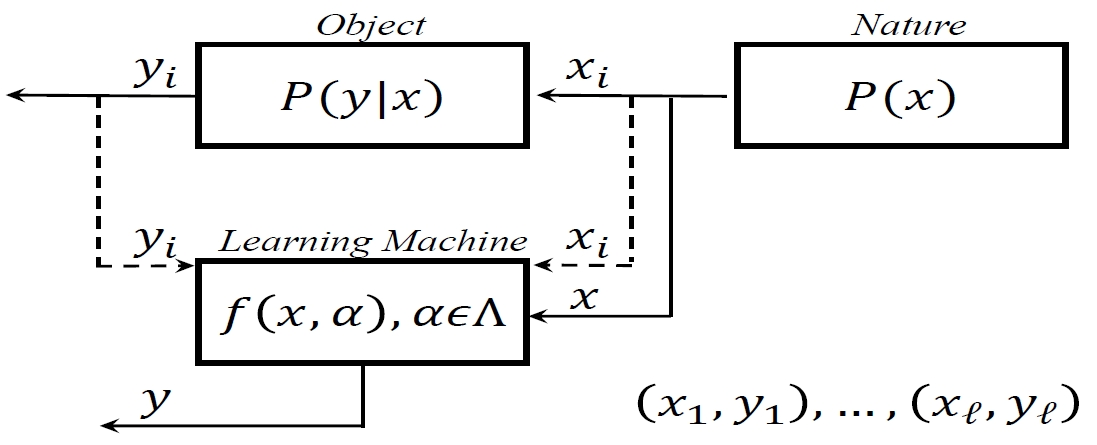
\includegraphics[width=.6\linewidth]{Imgs/slt.png}
\end{figure}

Given $\ell$ iid observations
\begin{align*}
(x_{1}, y_{1}), \ldots, (x_{\ell}, y_{\ell}), x \in X, y \subset \{0, 1\}
\end{align*}
generated by unknown $P(x, y) = P(y|x)P(x)$, find the rule
\begin{align*}
r(x) = \theta(f_{0}(x)),
\end{align*}
which minimizes in a set $\{f(x)\}$ probability if misclassification
\begin{align*}
R_{\theta }(f) = \int |y - \theta(f(x))|dP(x,y)
\end{align*}
\end{frame}

\begin{frame}{STANDARD REPLACEMENT OF BASIC SETTING}
Using data
\begin{align*}
(x_{1}, y_{1}), \ldots, (x_{\ell}, y_{\ell}), x \in X, y \subset \{0, 1\}
\end{align*}
minimize in the set of functions $\{f(x)\}$ the functional
\begin{align*}
R(f) = \int (y - f(x))^{2}dP(x, y)
\end{align*}
(instead of functional $R_{\theta}(f) = \int |y - \theta(f(x))|dP(x, y)$).

Minimizer $f_{0}(x)$ of $R(f)$ estimates conditional probability function $f_{0}(x) = P(y=1|x)$. Use the classification rule
\begin{align*}
r(x) = \theta(f_{0}(x) - 0.5) = \theta(P(y = 1|x) - 0.5).
\end{align*}
\end{frame}

\begin{frame}{PROBLEM WITH STANDARD REPLACEMENT}
Minimization of functional $R(f)$ in the set $\{f(x)\}$ is equivalent to minimization of the expression
\begin{align*}
R(f) &= \int (y - f(x))^{2}dP(x, y)\\
&= \int \left[(y - f_{0}(x)) + (f_{0}(x) - f(x)) \right]^{2}dP(x, y)
\end{align*}
where $f_{0}(x)$ minimizes $R(f)$. This is equivalent to minimization
\begin{align*}
R(f) &= \int (y - f_{0}(x))dP(x, y) + \\
&\int (f_{0}(x) - f(x))^{2}dP(x) + 2\int (y - f_{0}(x))(f_{0}(x)-f(x))dP(x,y).
\end{align*}

\begin{center}
\textbf{ACTUAL GOAL IS: USING $\ell$ OBSERVATIONS TO MINIMIZE THE SECOND INTEGRAL, {\color{blue}{NOT SUM OF LAST TWO INTEGRALS}}}.
\end{center}
\end{frame}


\begin{frame}{DIRECT ESTIMATION OF CONDITIONAL PROBABILITY}
\begin{enumerate}
\item When $y \subset \{0, 1\}$ the conditional probability $P(y=1|x)$ is defined by some real valued function $0 \leq f(x) \leq 1$.
\item From Bayesian formula
\begin{align*}
P(y=1|x)p(x) = p(y=1,x)
\end{align*}
follows that any function $G(x - x^{\prime}) \in L_{2}$ defines equation
\begin{align*}
\int G(x-x^{\prime})f(x^{\prime})dP(x^{\prime}) = \int G(x-x^{\prime})dP(y=1, x^{\prime}) \quad (*)
\end{align*}
which solution is conditional probability $f(x) = P(y=1|x)$.
\item To estimate conditional probability means to solve the equation (*) when $P(x)$ and $P(y=1, x)$ are unknown but iid data,
\begin{align*}
(x_{1}, y_{1}), \ldots, (x_{1}, y_{\ell})
\end{align*}
generated according to $P(y, x)$, are \emph{given}.
\item Solution of equation (*) is ill-posed problem.
\end{enumerate}
\end{frame}


\begin{frame}{MAIN INDUCTIVE STEP IN STATISTICS}
Replace the unknown Cumulative Distribution Function (CDF) $P(x), x = (x^{1}, \ldots, x^{n})^{T} \in R^{n}$ with it estimate $P_{\ell}(x)$: The Empirical Cumulative Distribution Function (ECDF)
\begin{align*}
P_{\ell}(x) = \frac{1}{\ell}\sum_{i=1}^{\ell}\theta\{x - x_{i}\}, \theta\{x - x_{i}\} = \prod_{k=1}^{n}\theta\{x^{k} - x_{i}^{k}\}
\end{align*}
obtained from data
\begin{align*}
x_{1}, \ldots, x_{\ell}, x_{i} = (x_{i}^{1}, \ldots, x_{i}^{n})^{T}.
\end{align*}
The main theorem of statistics claims that ECDF convergences to actual CDF \emph{uniformly} with fast rate of convergence. The following inequality holds true
\begin{align*}
P\{\sup_{x}^{} |P(x) - P_{\ell}(x)| > \epsilon\} < 2\exp\{-2\epsilon^{2}l\}, \quad \forall \epsilon.
\end{align*}
\end{frame}


\begin{frame}{TWO CONSTRUCTIVE SETTINGS OF CLASSIFICATION PROBLEM}
\begin{enumerate}
\item \emph{Standard constructive setting:} Minimization of functional
\begin{align*}
R_{\text{emp}}(f) = \int (y - f(x))^{2}dP_{\ell}(x, y),
\end{align*}
in a set $\{f(x)\}$ using data $(x_{1}, y_{1}), \ldots, (x_{\ell}, y_{\ell})$ leads to
\begin{align*}
R_{\text{emp}}(f) = \frac{1}{\ell}\sum_{i=1}^{\ell}(y_{i} - f(x_{i}))^{2}, \quad f(x) \in \{f(x)\}.
\end{align*}
\hrulefill
\item \emph{New constructive setting:} Solution of equation
\begin{align*}
\int G(x - x^{\prime})f(x^{\prime})dP_{\ell}(x^{\prime}) = \int G(x - x^{\prime})dP_{\ell}(y = 1, x^{\prime}),
\end{align*}
using data leads to solution in $\{f(x)\}$ the equation
\begin{align*}
\frac{1}{\ell}\sum_{i=1}^{\ell}G(x-x_{i})f(x_{i}) = \frac{1}{\ell}\sum_{j=1}^{\ell}y_{j}G(x-x_{j}), \quad f(x) \in \{f(x)\}.
\end{align*}
\end{enumerate}
\end{frame}

\begin{frame}{NADARAYA-WATSON ESTIMATOR OF CONDITIONAL PROBABILITY}
It is known Nadaraya-Watson estimator of $P(y=1|x)$:
\begin{align*}
f(x) = \frac{\sum_{i=1}^{\ell}y_{i}G(x-x_{i})}{\sum_{i=1}^{\ell}G(x-x_{i})}
\end{align*}
where special kernels $G(x-x_{i})$ (say, Gaussian) are used.

This estimator is the solution of "corrupted" equation
\begin{align*}
\frac{1}{\ell}\sum_{i=1}^{\ell}G(x-x_{i})f(x) = \frac{1}{\ell}\sum_{i=1}^{\ell}y_{i}G(x-x_{i})
\end{align*}
(which uses special kernel) rather than the obtained equation
\begin{align*}
\frac{1}{\ell}\sum_{i=1}^{\ell}G(x-x_{i})f(x_{i}) = \frac{1}{\ell}\sum_{j=1}^{\ell}y_{i}G(x-x_{j})
\end{align*}
(which is defined for any kernel $G(x-x^{\prime})$ from $L_{2}$).
\end{frame}


\begin{frame}{WHAT MEANS TO SOLVE THE EQUATION}
To solve the equation
\begin{align*}
\frac{1}{\ell}\sum_{i=1}^{\ell}G(x-x_{i})f(x_{i}) = \frac{1}{\ell}\sum_{j=1}^{\ell}y_{j}G(x-x_{j})
\end{align*}
means to find the function in $\{f(x)\}$ minimizing $L_{2}$-distance
\begin{align*}
R(f) = \int \left( \sum_{i=1}^{\ell}G(x-x_{i})f(x_{i}) - \sum_{j=1}^{\ell}y_{j}G(x-x_{j}) \right)^{2}d\mu(x)
\end{align*}
Simple algebra leads to expression
\begin{align*}
R_{\mathcal{V}}(f) = \sum_{i,j = 1}^{\ell}(y_{i} - f(x_{i}))(y_{j} - f(x_{j}))v(x_{i}, x_{j}),
\end{align*}
where values $v(x_{i}, x_{j})$ are
\begin{align*}
v(x_{i}, x_{j}) = \int G(x-x_{i})G(x-x_{j})d\mu(x), \quad i,j=1,\ldots,l.
\end{align*}
Values $v(x_{i}, x_{j})$ form $\mathcal{V}$-matrix.
\end{frame}


\begin{frame}{THE $\mathcal{V}$-MATRIX ESTIMATE}
\begin{enumerate}
\item For $\mu(x) = P(x)$ elements $v(x_{i}, x_{j})$ of $\mathcal{V}$-matrix are
\begin{align*}
v(x_{i}, x_{j}) = \int G(x-x_{i})G(x-x_{j})dP(x).
\end{align*}
Using empirical estimate $P_{\ell}(x)$ instead of $P(x)$ we obtain the following estimates of elements of $\mathcal{V}$-matrix
\begin{align*}
v(x_{i}, x_{j}) = \frac{1}{\ell}\sum_{s=1}^{\ell}G(x_{s} - x_{i})G(x_{s} - x_{j})
\end{align*}
\item For $\mu(x) = x, x \in (-1, 1)$ and $G(x-x^{\prime}) = \exp\{-0.5\delta^{2}(x-x^{\prime})^{2}\}$,
\begin{align*}
&v(x_{i}, x_{j}) = \\ 
&\exp\{-\delta^{2}(x_{i}- x_{j})^{2}\}\\
&\{erf[\delta(1+0.5(x_{i}+x_{j}))] + erf[\delta(1-0.5(x_{i}+x_{j}))]\}
\end{align*}
\end{enumerate}
\end{frame}


\begin{frame}{LEAST $\mathcal{V}$-QUADRATIC FORM METHOD AND LEAST SQUARES METHOD}
Let $(x_{1}, y_{1}), \ldots, (x_{\ell}, y_{\ell})$ be training data. Using notations:
\begin{align*}
Y = (y_{1}, \ldots, y_{\ell})^{T}, \quad F(f) = (f(x_{1}), \ldots, f(x_{\ell}))^{T}, \ldots, \mathcal{V} = ||v(x_{i}, x_{j})|| 
\end{align*}
we can rewrite functional
\begin{align*}
R_{\mathcal{V}}(f) = \sum_{i,j=1}^{\ell}(y_{i}-f(x_{i}))(y_{j}-f(x_{j}))v(x_{i}, x_{j}),
\end{align*}
in matrix form
\begin{align*}
R_{\mathcal{V}}(f) = (y - F(f))^{T}\mathcal{V}(y - F(f)).
\end{align*}
We call this functional \emph{Least $\mathcal{V}$-quadratic} functional.

Identity matrix $\mathcal{I}$ instead of $\mathcal{V}$ forms \emph{Least Squares} functional
\begin{align*}
R_{I}(f) = (Y - F(f))^{T}(Y - F(f)).
\end{align*}
\end{frame}

\section{PART III: SELECTION OF ADMISSIBLE SET OF FUNCTIONS}
\begin{frame}
{\color{blue}{
\begin{center}
PART III
\end{center}
\begin{center}
SELECTION OF ADMISSIBLE SET OF FUNCTIONS
\end{center}
}}
\end{frame}

\begin{frame}{STRONG AND WEAK CONVERGENCE}
Functions $f_{\ell}(x) \in L_{2}$ have two modes of convergence:
\begin{enumerate}
\item Strong mode of convergence (convergence of functions)
\begin{align*}
\lim_{l \rightarrow \infty} \int (f_{\ell}(x) - f_{0}(x))^{2}d\mu(x) = 0.
\end{align*}
\item Weak mode of convergence (convergence of functionals)
\begin{align*}
\lim_{l \rightarrow \infty} \int f_{\ell}(x)\phi(x)d\mu(x) = \int f_{0}(x)\phi(x)d\mu(x), \quad \forall \phi(x) \in L_{2}\\
(\text{convergence for all possible functions} \phi(x) \in L_{2})
\end{align*} 
\item[•] Strong mode of convergence implies weak convergence:
\begin{align*}
\left( \int (f_{\ell}(x) - f_{0}(x))\phi(x)d\mu(x) \right)^{2} \leq \int (f_{\ell}(x) - f_{0}(x))^{2}d\mu(x) \int \phi^{2}(x)\mu(x).
\end{align*}
\item[•] For functions $f_{\ell}(x)$ belonging to compact ewak mode of convergence implies strong mode of convergence.
\end{enumerate}
\end{frame}

\begin{frame}{WEAK CONVERGENCE TO CONDITIONAL PROBABILITY FUNCTIONS $P(y=1|x)$}
Weak mode convergence of sequence of functions $f_{\ell}(x)$ to function $f_{0}(x) = P(y=1|x)$ means equalities
\begin{align*}
\lim_{l \rightarrow \infty} \int \phi(x)f_{\ell}(x)dP(x) &= \int \phi(x)P(y=1|x)dP(x)\\
&= \int \phi(x)dP(y=1,x)
\end{align*} 
for all $\phi(x) \in L_{2}$.

Let us call set of $m$ functions $\phi_{1}(x), \ldots, \phi_{m}(x)$ from $L_{2}$ the \emph{chosen predicates}. Let us call subset of functions $\{f(x)\}$ for which the following $m$ equalities hold true
\begin{align*}
\int \phi_{k}(x)f(x)dP(x) = \int \phi_{k}(x)dP(y=1, x), \quad k = 1, \ldots, m,
\end{align*}
the \emph{admissible set of functions (defined by the predicates)}.
\end{frame}


\begin{frame}{ADMISSIBLE SUBSETS FOR ESTIMATION CONDITIONAL PROBABILITY FUNCTION}
Replacing $P(x), P(y=1, x)$ with $P_{\ell}(x), P_{\ell}(y=1, x)$ we obtain
\begin{align*}
\frac{1}{\ell}\sum_{i=1}^{\ell}\phi_{k}(x_{i})f(x_{i}) = \frac{1}{\ell}y_{i}\phi_{k}(x_{i}), \quad k = 1,\ldots, m.
\end{align*}
In the matrix notations
\begin{align*}
Y = (y_{1}, \ldots, y_{\ell})^{T}, F(f) = (f(x_{1}), \ldots, f(x_{\ell}))^{T}, \Phi_{k} = (\phi_{k}(x_{1}), \ldots, \phi_{k}(x_{\ell}))^{T}.
\end{align*}
we obtain that:

\emph{The admissible set of functions $\{f(x)\}$ satisfies equalities}
\begin{align*}
\Phi_{k}^{T}F(f) = \Phi_{k}^{T}Y, \quad k = 1, \ldots, m.
\end{align*}
We call these equalities \emph{statistical invariants for} $P(y=1|x)$.
\end{frame}

\begin{frame}{DUCK TEST,STATISTICAL INVARIANTS, PREDICATES, AND FEATURES}

\centering{\color{blue}{THE DUCK TEST LOGIC}}

"If it looks like a duck, swims like a duck, and quacks like a duck, then it probably is a duck." (English proverb.)

\centering{\color{blue}{STATISTICAL INVARIANTS}}
\begin{align*}
\frac{1}{\ell}\sum_{i=1}^{\ell}\phi_{k}(x_{i})f(x_{i}) = \frac{1}{\ell}\sum_{i=1}^{\ell}y_{i}\phi_{k}(x_{i}), \quad k = 1, \ldots, m,
\end{align*}
(or $\Phi_{k}^{T}F(f) = \Phi_{k}^{T}Y, k = 1, \ldots, m$ in vector notations)

collect set of admissible functions $\{f(x)\}$ which "identify" animal as a duck if it "looks, swims, and quacks like a duck".

\centering{\color{blue}{PREDICATES AND FEATURES}}

Concepts of predicates and features are very different"
\begin{enumerate}
\item[•] With increasing number of predicates the VC-dimension of admissible set of functions $\{f(x)\}$ {\color{blue}{DECREASES}}.
\item[•] With increasing number of features the VC-dimension of admissible set of functions $\{f(x)\}$ {\color{blue}{INCREASES}}.
\end{enumerate}
\end{frame}


\begin{frame}{EXACT SETTING OF COMPLETE LEARNING PROBLEM}
\begin{enumerate}
\item[•] The complete solution of classification problem requires:

\emph{in a given set of functions $\{f(x)\}$ to minimize functional}
\begin{align*}
R_{\mathcal{V}}(f) = (Y - F(f))^{T}\mathcal{V}(Y - F(f)),
\end{align*}
\emph{subject to constraints (statistical invariants)}
\begin{align*}
\Phi_{k}^{T}F(f) = \Phi_{k}^{T}Y, \quad k = 1, \ldots, m.
\end{align*}

We call this conditional minimization model of learning
\centering{\emph{Learning Using Statistical Invariants}(LUSI)}
\item[•] Classical methods require in a given (\emph{specially constructed}) subset of functions $\{f(x)\}$ to minimize the functional
\begin{align*}
R_{\mathcal{I}}(f) = (Y - F(f))^{T}(Y - F(f)).
\end{align*}
\end{enumerate}
\end{frame}

\begin{frame}{APPROXIMATE SETTING OF COMPLETE LEARNING PROBLEM}
In this setting minimization of the functional
\begin{align*}
R_{\mathcal{V}}(f) = (Y - F(f))^{T}\mathcal{V}(Y - F(f)),
\end{align*}
on the set of functions $\{f(x)\}$ satisfying $m$ constraints
\begin{align*}
\Phi_{s}^{T}F(f) = \Phi_{s}^{T}Y, \quad s = 1, \ldots, m
\end{align*}
is replaced with minimization of the functional
\begin{align*}
R_{\mathcal{VP}}(f) = \hat{\tau}(Y - F(f))^{T}\mathcal{V}(Y - F(f)) + \frac{\tau}{m}\sum_{s=1}^{m}(\Phi_{s}^{T}F(f) - \Phi_{s}^{T}Y)^{2},
\end{align*}
where $\hat{\tau}, \tau \geq 0, \hat{\tau} + \tau = 1$. This functional can be rewritten as
\begin{align*}
R_{\mathcal{VP}}(f) = (Y - F(f))^{T}(\hat{\tau}\mathcal{V} + \tau\mathcal{P})(Y - F(f)),
\end{align*}
where $(l \times l)$ matrix $\mathcal{P}$ defines predicates convariance
\begin{align*}
\mathcal{P} = \frac{1}{m}\sum_{s=1}^{m}\Phi_{s}\Phi_{s}^{T}.
\end{align*}
\end{frame}


\section{PART IV: COMPLETE SOLUTION IN REPRODUCING KERNEL HILBERT SPACE (RKHS)}
\begin{frame}
{\color{blue}{
\begin{center}
PART IV
\end{center}
\begin{center}
COMPLETE SOLUTION IN REPRODUCING KERNEL HILBERT SPACE (RKHS)
\end{center}
}}
\end{frame}


\begin{frame}{IMPORTANT FACTS FROM RKHS 1.}
\begin{enumerate}
\item RKHS is set of functions $\{f(x)\}$ for which
\begin{align*}
(K(x, x^{\prime}), f(x^{\prime})) = f(x), \quad (K(x, x^{\prime}) \text{ is Mercer kernel}).
\end{align*}
\item Mercer kernel is defined by orthonormal functions $\psi_{k}(x)$
\begin{align*}
K(x, x^{\prime}) = \sum_{i=1}^{\infty}\lambda_{i}\psi_{i}(x)\psi_{i}(x^{\prime}), \quad \lambda_{i} > 0, \lambda_{t} \rightarrow_{t \rightarrow \infty} = 0.
\end{align*}
\item Set of functions
\begin{align*}
f_{c}(x) = \sum_{i=1}^{\infty}c_{i}\psi_{i}(x)
\end{align*}
with inner product (and norm)
\begin{align*}
(f_{c}(x), f_{c^{*}}(x)) = \sum_{i=1}^{\infty}\frac{c_{i}c_{i}^{*}}{\lambda_{i}} \left( ||f_{c}(x)||^{2} = \sum_{i=1}^{\infty}\frac{c_{i}^{2}}{\lambda_{i}} \right)
\end{align*}
forms RKHS of kernel $K(x, x^{\prime})$.
\end{enumerate}
\end{frame}


\begin{frame}{IMPORTANT FACTS FROM RKHS 2.}
\begin{enumerate}
\item[4.] \textbf{REPRESENTER THEOREM.} Minimum of functional
\begin{align*}
R_{\mathcal{V}}(f) = (Y - F(f))^{T}\mathcal{V}(Y - F(f))
\end{align*}
in subset of RKHS with $||f(x)||^{2} \leq C$ has representation
\begin{align*}
f_{0}(x) = \sum_{i=1}^{\ell}a_{t}K(x_{i}, x) = A^{T}\mathcal{K}(x), \quad (*)
\end{align*}
where $A = (a_{1}, \ldots, a_{\ell})^{T}$, $\mathcal{K}(x) = (K(x_{1}, x), \ldots, K(x_{\ell}, x))^{T}$.
\item[5.] Square of norm of function $f(x)$ in form (*) is
\begin{align*}
||f(x)||^{2} = A^{T}KA, \quad K = ||K(x_{i}, x_{j})||, \quad F(f) = KA.
\end{align*}
\item[6.] Sunset of functions from RKHS with bounded norm $A^{T}KA \leq C$ has finite VC-dimension (the smaller $C$, the smaller is VC-dimension). By controlling $C$, one control both: the VC dimension of subset of functions and their smoothness.

\centering{\emph{Structure defined by C is the key in implementation SRM principle for functions belonging to RKHS.}}
\end{enumerate}
\end{frame}

\begin{frame}{CONDITIONAL MINIMIZATION IN RKHS: EXACT LUSI SOLUTION}
For RKHS we have $F(f) = KA$. Minimum of the functional
\begin{align*}
R_{\mathcal{V}}(f) = (KA-Y)^{T}\mathcal{V}(KA-Y),
\end{align*}
subject to $m$ constraints
\begin{align*}
\Phi_{k}^{T}KA = \Phi_{k}^{T}Y, \quad k = 1, \ldots, m
\end{align*}
and constraint
\begin{align*}
A^{T}KA \leq C
\end{align*}
has unique solution of the form $f_{\ell}(x) = A_{\text{LUSI}}^{T}\mathcal{K}(x)$, where
\begin{align*}
A_{\text{LUSI}} = A_{\mathcal{V}} - \sum_{s=1}^{m}\mu_{s}A_{s},
A_{\mathcal{V}} = (\mathcal{V}K + \gamma_{c}I)^{-1}\mathcal{V}Y, A_{s} = (\mathcal{V}K + \gamma_{c}I)^{-1}\Phi_{s}
\end{align*}
Parameters $\mu_{s}$ are solution of linear equations
\begin{align*}
\sum_{s=1}^{m}\mu_{s}A_{s}^{T}K\Phi_{s} = (KA_{\mathcal{V}} - Y)^{T}\Phi_{s}, \quad s = 1,\ldots, m.
\end{align*}
\end{frame}

\begin{frame}{UNCONDITIONAL MINIMIZATION IN RKHS (SOLUTION OF APPROXIMATE SETTING)}
Minimum of functional
\begin{align*}
R_{\mathcal{VP}}(f) = (KA - Y)^{T}(\hat{\tau}\mathcal{V} + \tau\mathcal{P})(KA - Y)
\end{align*}
in the set of functions $\{f(x)\}$ belonging to RKHS of kernel $K(x,x^{\prime})$ with bounded norm
\begin{align*}
A^{T}KA \leq C
\end{align*}
has unique solution of the form
\begin{align*}
f_{0}(x) = A_{\mathcal{VP}}^{T}\mathcal{K}(x),
\end{align*}
where
\begin{align*}
A_{\mathcal{VP}} = ((\hat{\tau}\mathcal{V} + \tau\mathcal{P})K + \gamma_{c}I)^{-1}(\hat{\tau}\mathcal{V} + \tau\mathcal{P})Y.
\end{align*}
\end{frame}

\begin{frame}{SVM AND LUSI-SVM ESTIMATIONS IN RKHS}
\begin{enumerate}
\item[•] \textbf{SVM:} Given data
\begin{align*}
(x_{1}, y_{1}), \ldots, (x_{\ell}, y_{\ell})
\end{align*}
find in RKHS the function $f(x) = A^{T}\mathcal{K}(x)$ with norm
\begin{align*}
||f(x)||^{2} = A^{T}KA \leq C \quad (*)
\end{align*}
that minimizes losses
\begin{align*}
L(A) = \sum_{i=1}^{\ell}|y_{i} - A^{T}\mathcal{K}(x_{i})|
\end{align*}
\item[•] \textbf{LUSI-SVM:} Given data find in RKHS the function $f(x) = A^{T}\mathcal{K}(x)$ with bounded norm (*) that minimizes
\begin{align*}
L(A) = \tau\sum_{s=1}^{m}|A^{T}K\Phi_{s} - Y^{T}\Phi_{s}| + \hat{\tau}\sum_{i=m+1}^{m+l} |y_{i} - A^{T}\mathcal{K}(x_{i})|,
\end{align*}
where $\tau + \hat{\tau} = 1, \tau > 0, \hat{\tau} > 0$.
\end{enumerate}
\end{frame}


\begin{frame}{LUSI-SVM ESTIMATOR}
LUSI-SVM method selects in set $A^{T}KA \leq C$ the function
\begin{align*}
f(x) = \sum_{i=1}^{\ell}a_{i}K(x_{i}, x) = A^{T}\mathcal{K}(x),
\end{align*}
where $A = \sum_{t=1}^{m}\delta_{t}\Phi_{t} + \sum_{t=m+1}^{m+l}\delta_{t}\Phi_{t}$.

To find $\delta_{t}$ one has to maximize the functional
\begin{align*}
R(\delta) = \sum_{i=1}^{m+l}\delta_{i}\Phi_{s}^{T}Y - \frac{1}{2}\sum_{r,s=1}^{m+l}\delta_{r}^{T}K\Phi_{s}\delta_{s}
\end{align*}
subject to constraints
\begin{align*}
-\hat{\tau}\gamma_{c}^{*} \leq \delta_{t} \leq \hat{\tau}\gamma_{c}^{*}, \quad t = (m+1), \ldots, (m+l),\\
-\tau\gamma_{c}^{*} \leq \delta_{t} \leq \tau\gamma_{c}^{*}, \quad t = 1, \ldots, m, \hat{\tau} + \tau = 1,
\end{align*}
where we denoted
\begin{align*}
\Phi_{m+t} = (0, \ldots, 1, \ldots, 0)^{T}, t = m+1, \ldots, m+l.
\end{align*}
\end{frame}

\begin{frame}{LEARNING DOES NOT REQUIRE BIG DATA}
According to Representer Theorem, the optimal solution of learning problem in RKHS have properties:
\begin{enumerate}
\item It is defined linear parametric functions in form of expansion on kernel functions (i.e optimal solution belongs to one layer network, not multi-layer network).
\item Observation vectors $x_{1},\ldots,x_{\ell}$ and kernel $K(x,x^{\prime})$ define basis of linear expansion for optimal $\ell$ parametric solution.
\item SVM: to control VC-dimension uses data to find both the basis of expansion and the parameters of solution.
\item LUSI-SVM: to estimate unknown parameters of solution, adds to $\ell$ training pairs $m$ pairs $(K\Phi_{s}, Y^{T}\Phi_{s})$ obtained using predicates. When $\tau \approx 1$ it uses just these $m$ pairs.
\item Since any functions from Hilbert space can be used as predicates $\phi_{s}(x)$, there exist one or several "smart" (actually "sophia") predicates defining pairs $(K\Phi_{s}, Y^{T}\Phi_{s})$ to form optimal solution.
\end{enumerate}
\end{frame}

\begin{frame}{ILLUSTRATION}
\begin{figure}
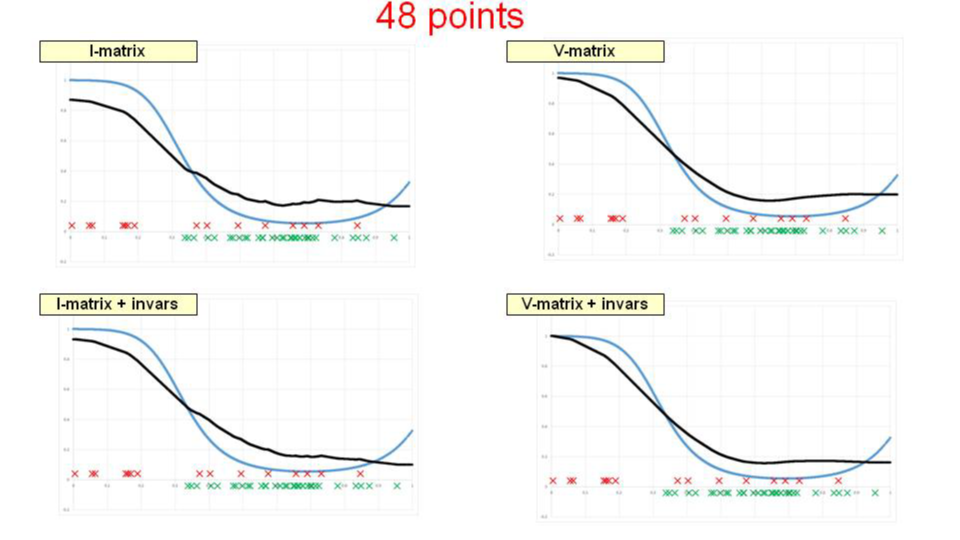
\includegraphics[width=1\linewidth]{Imgs/lusi-fig1.png}
I: 0.3756 \quad V:0.1432\\
I\&I: 0.2166 \quad V\&I: 0.1017
\end{figure}
\end{frame}

\begin{frame}{ILLUSTRATION}
\begin{figure}
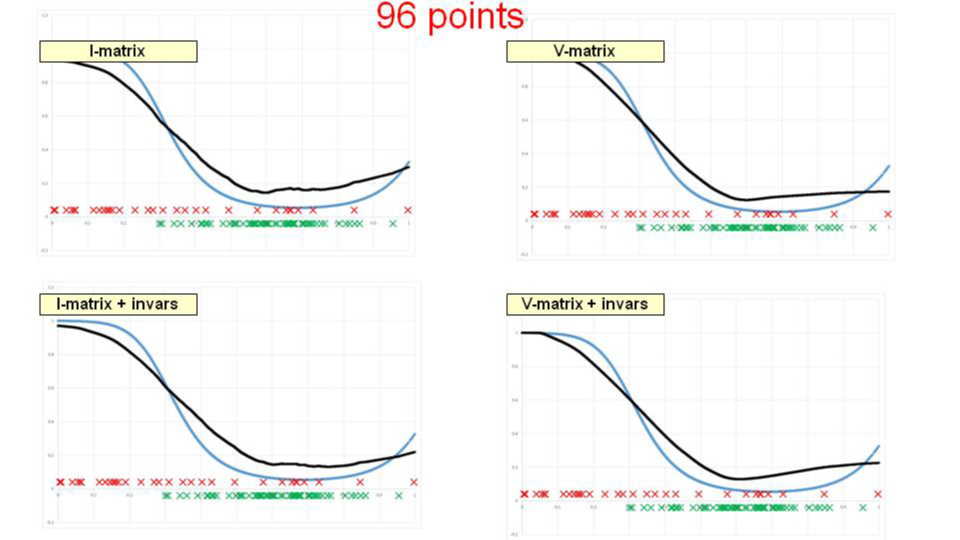
\includegraphics[width=1\linewidth]{Imgs/lusi-fig2.png}
I: 0.3212 \quad V:0.1207\\
I\&I: 0.1808 \quad V\&I: 0.0778
\end{figure}
\end{frame}

\begin{frame}{ILLUSTRATION}
\begin{figure}
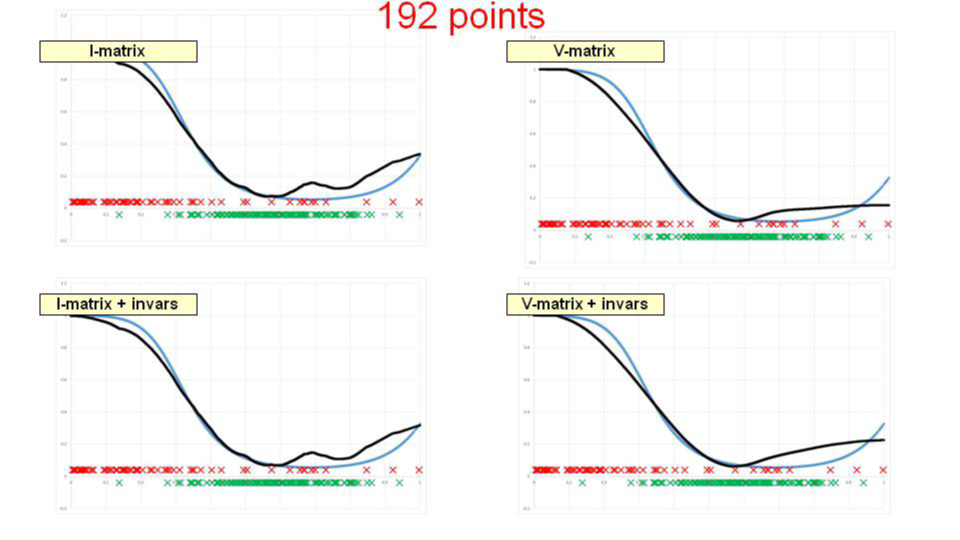
\includegraphics[width=1\linewidth]{Imgs/lusi-fig3.png}
I: 0.1672 \quad V:0.0689\\
I\&I: 0.1072 \quad V\&I: 0.0609
\end{figure}
\end{frame}

\begin{frame}{MULTIDIMENSIONAL EXAMPLES}
\begin{figure}
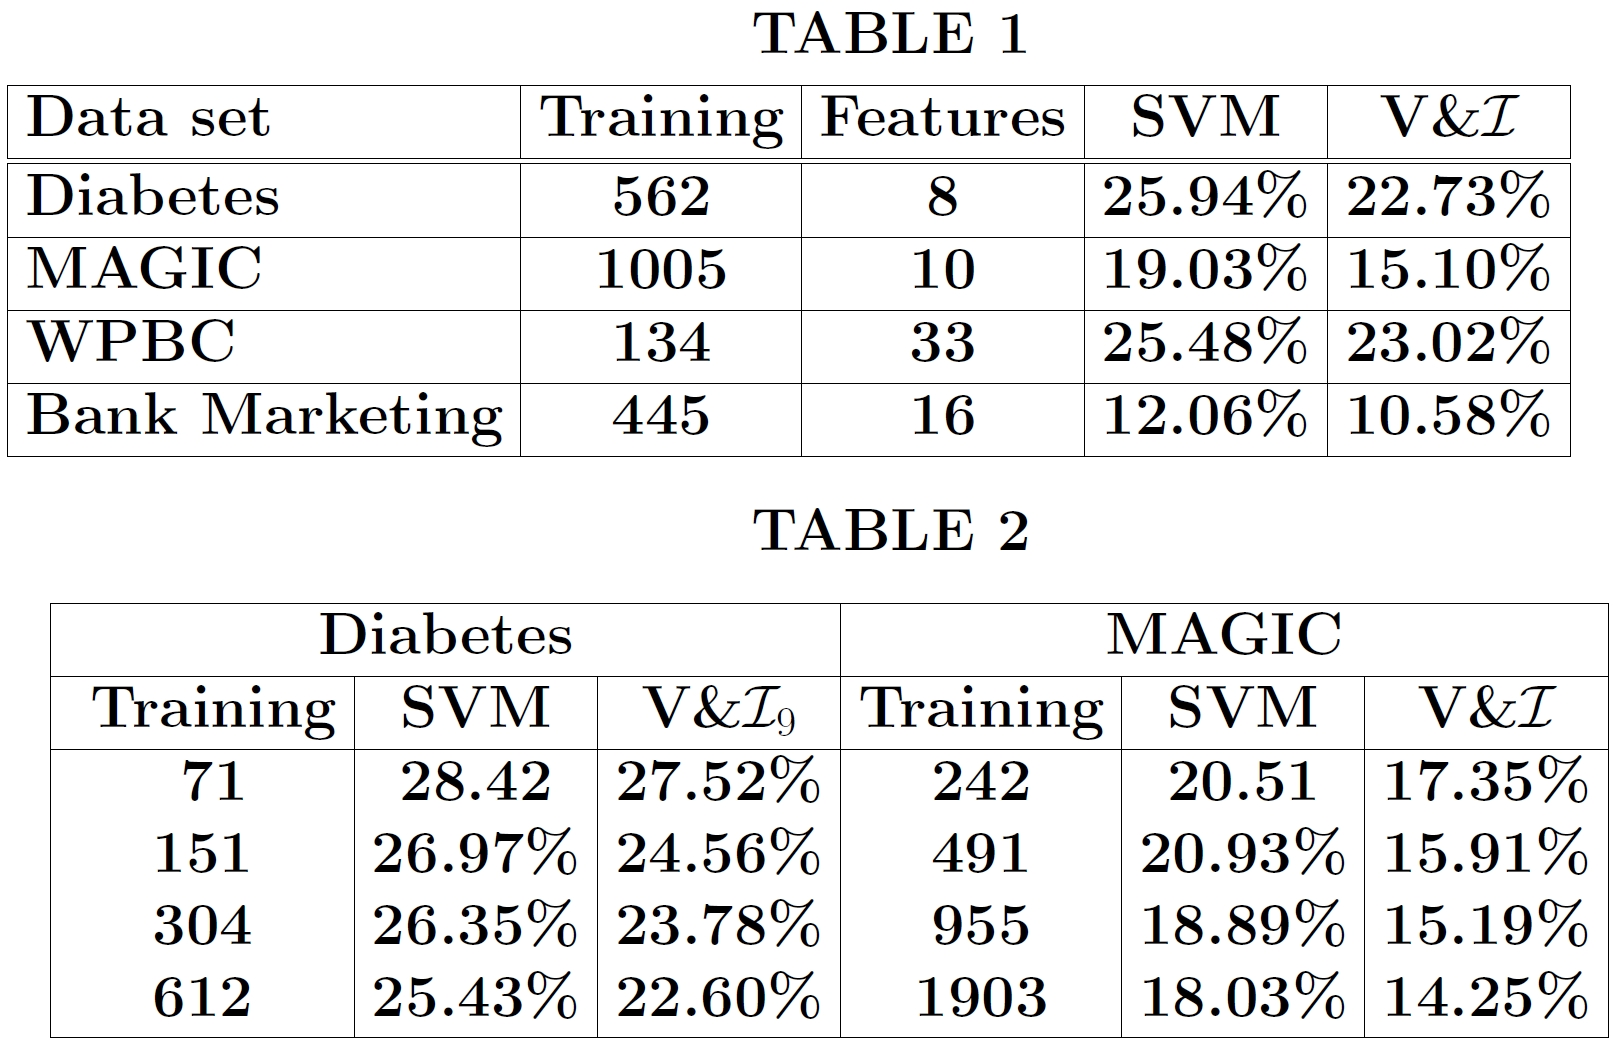
\includegraphics[width=.8\linewidth]{Imgs/table1and2.png}
\end{figure}
\end{frame}

\begin{frame}{NEW INVARIANT FOR DIABETES}
\begin{figure}
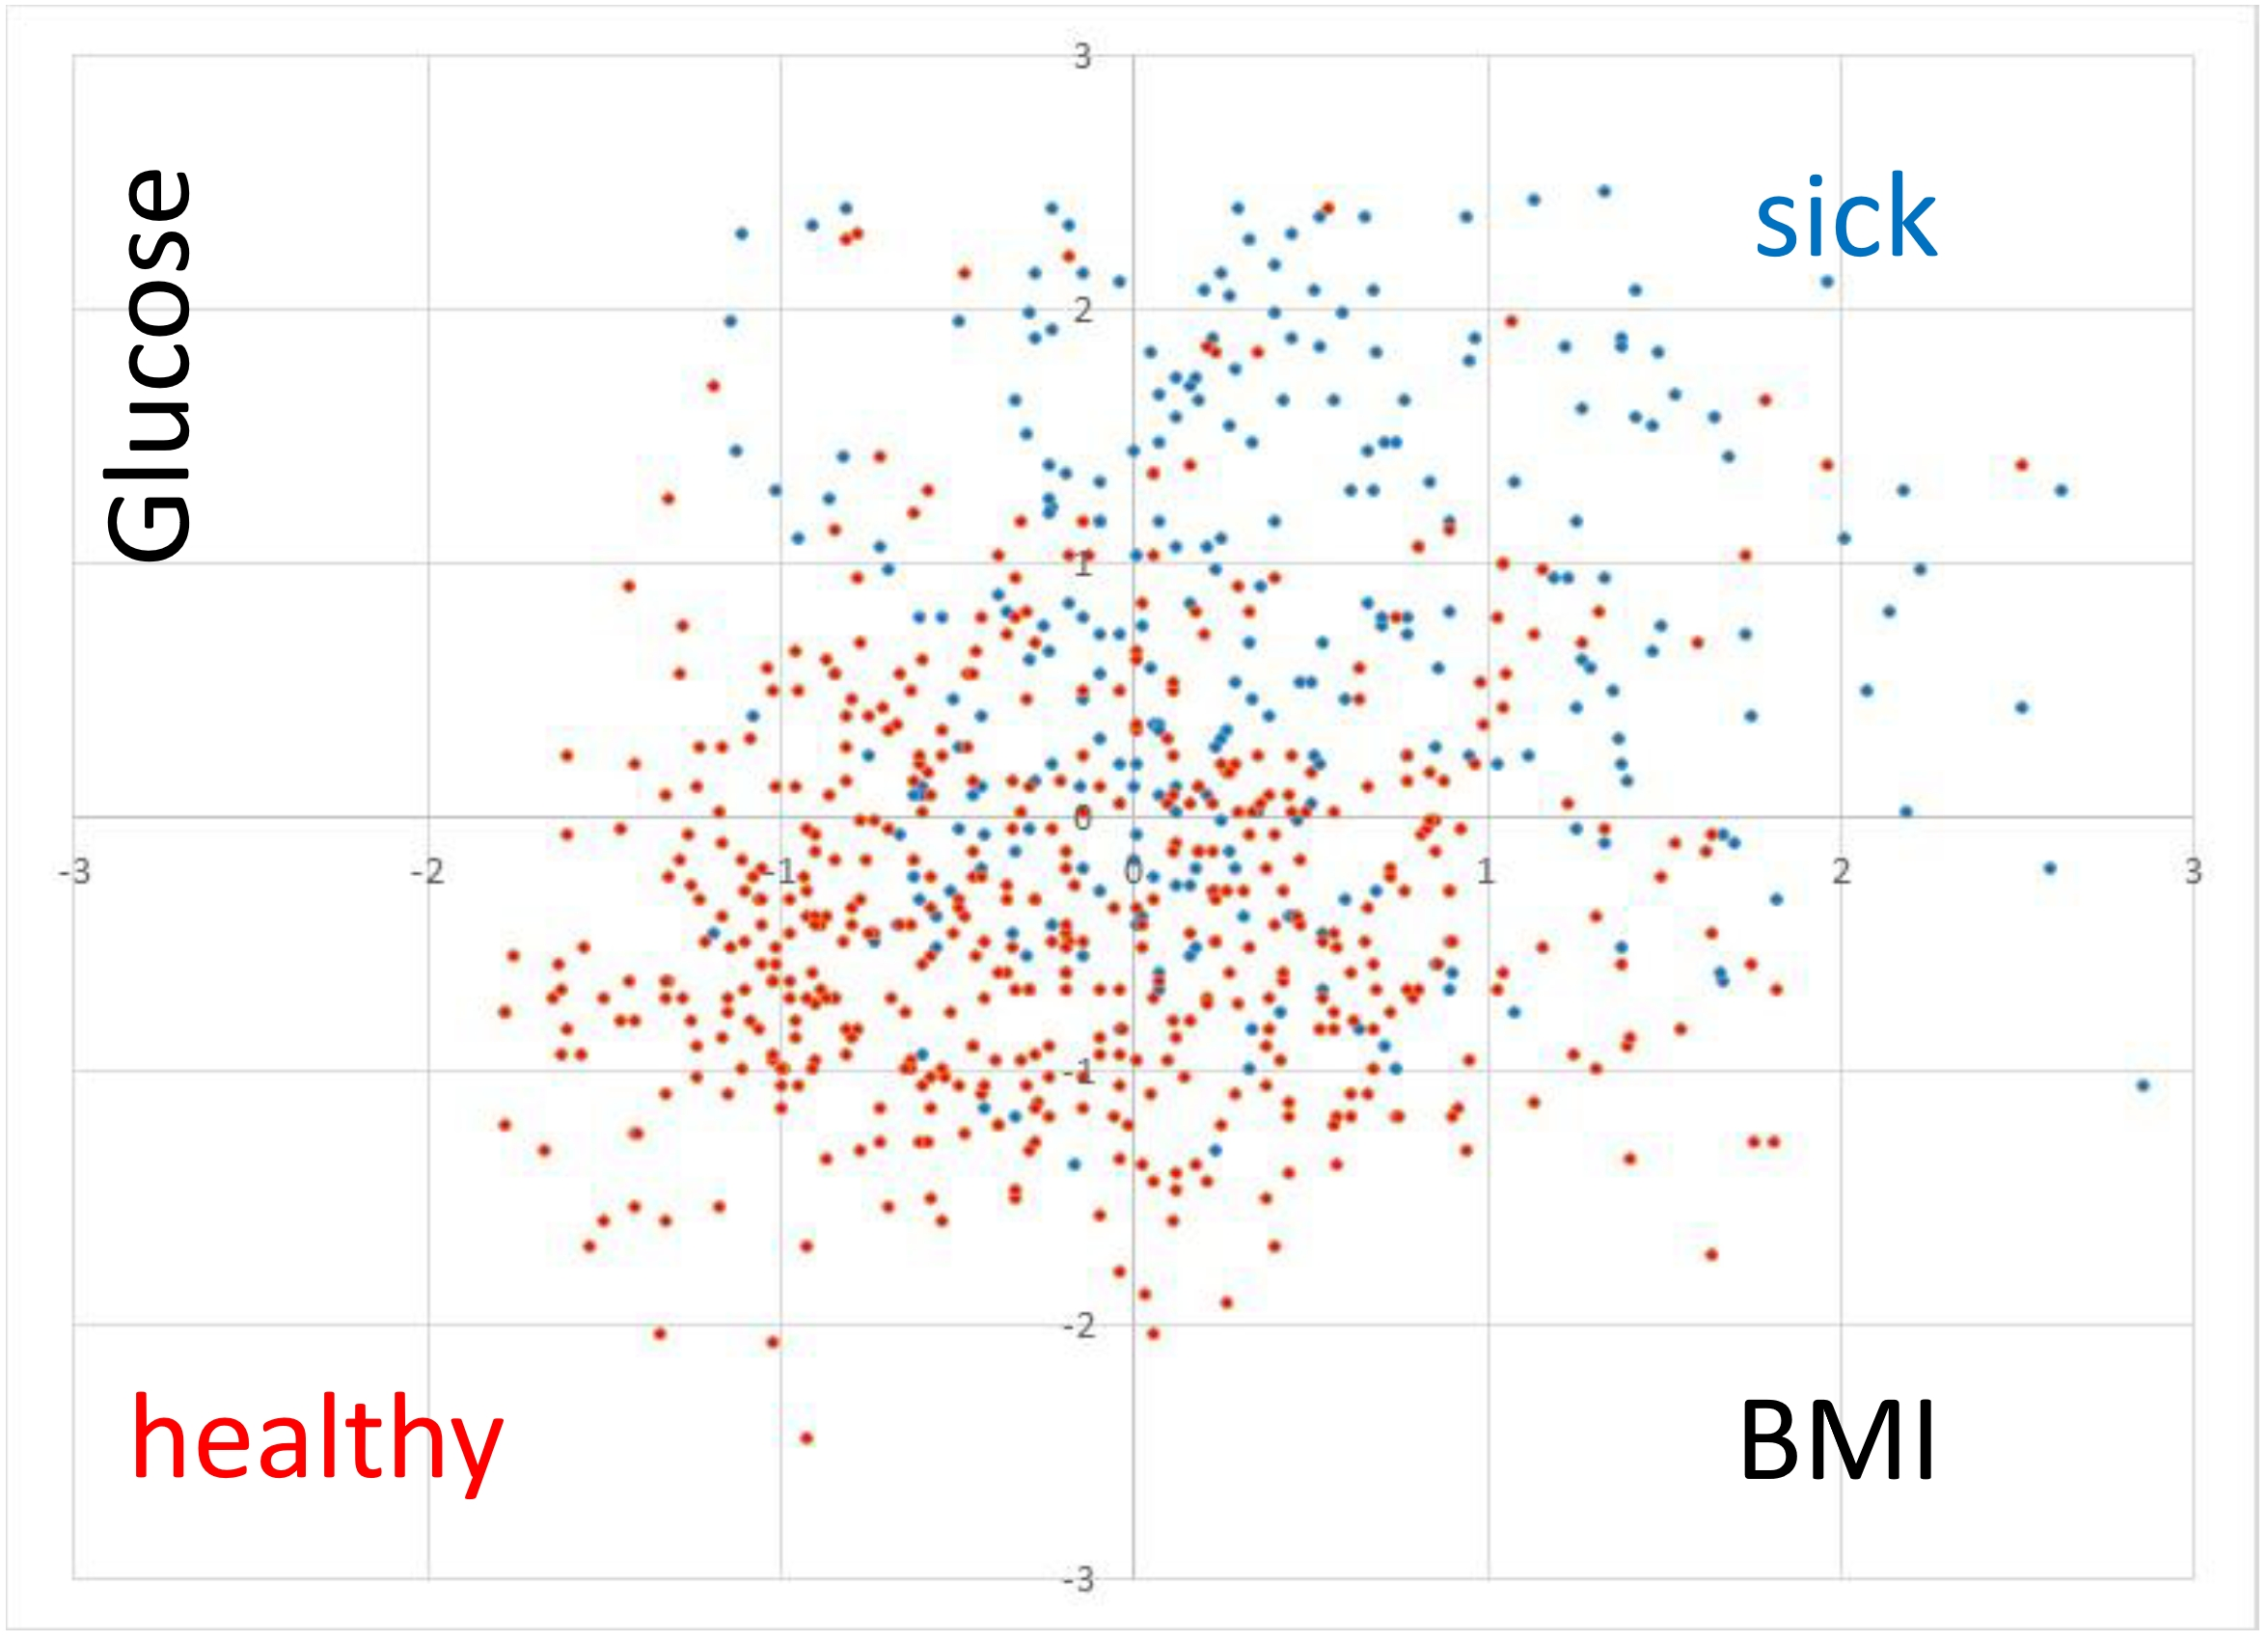
\includegraphics[width=.8\linewidth]{Imgs/BMI-Glucose-for-ylable(healthy-vs-sick).png}
I\&$\mathcal{I}_{+*}$ decreases errors rate from 22.73\% to 22.07\%.
\end{figure}
\end{frame}

\begin{frame}{WAY TO FIND NEW INVARIANT}
\emph{Find a situation (the box $\mathcal{B}$ in Fig.), where the existing solution (the approximation $P_{\ell}(y=1|x)$) contradicts the evidence (contradicts invariant for predicate $\phi(x) = 1$ inside the box) and then modify the solution (obtain a new approximation $P_{n+1}(y=1|x)$) which resolves this contradiction.}

\hrulefill

This is the same principle  that used in Physics to discover the laws of Nature. To discover laws of the Nature physicists first trying to find a situation where existing theory contradicts observations (The invariants fail. Theoretical predictions do not supported by experiments). Then they trying to reconstruct theory to remove the contradictions. They construct a new approximation of theory which does not contradict the observed reality —— keeps all invariants.

\hrulefill

\centering{\emph{The most important (and most difficult) part in scientific discovery is to find contradictive situation.}}
\end{frame}

\section{PART V: LUSI APPROACH IN NEURAL NETWORKS}
\begin{frame}
{\color{blue}{
\begin{center}
PART V
\end{center}
\begin{center}
LUSI APPROACH IN NEURAL NETWORKS
\end{center}
}}
\end{frame}


\begin{frame}{$\mathcal{VP}$-BACK PROPAGATION ALGORITHM}
\begin{enumerate}
\item[•] Neural Networks searching for minimum of functional
\begin{align*}
R_{\mathcal{I}}(f) = (F(f) - Y)^{T}(F(f) - Y),
\end{align*}
in the set of piece-wise linear functions $\{f\}$ realized by neural network. It uses gradient descent procedure of minimization (called \emph{Back Propagation}). Procedure has three steps: 1. Forward propagation. 2. Backward propagation. 3. Updates of parameters.
\item[•] To minimize in the same set of functions the $\mathcal{VP}$-form
\begin{align*}
R_{\mathcal{VP}}(f) = (F(f) - Y)^{T}(\hat{\tau}\mathcal{V} + \tau\mathcal{P})(F(f) - Y),
\end{align*}
using back propagation technique, one has to modify just backward step: instead of vector $E = (y_{1}-u_{1}), \ldots, (y_{\ell}-u_{\ell})^{T}$, (where $u_{1}, \ldots, u_{\ell}$ are outputs of the last layer (last unit) on vector $x_{1}, \ldots, x_{\ell}$) one has back propagate modified vector
\begin{align*}
\hat{E} = (\hat{\tau}\mathcal{V} + \tau\mathcal{P})E.
\end{align*}
\end{enumerate}
\end{frame}


\begin{frame}{SCHEME OF $\mathcal{VP}$-BACK PROPAGATION ALGORITHM}
\begin{enumerate}
\item \emph{Forward propagation step.} Given initial weights $w$ of Net,  propagate training vectors $x_{i}$ through all hidden layers.
\item \emph{Border conditions for back propagation.} Let $u_{i}$ be value corresponding to vector $x_{i}$ propagated on the last layer (unit) and $e_{i} = (y_{i} - u_{i})$ be difference between target value $y_{i}$ and obtained value $u_{i}$. Consider vector $E = (e_{1}, \ldots, e_{\ell})^{T}$.
\item \emph{Back propagation step.} Back propagation vector
\begin{align*}
\hat{E} = (\hat{\tau}\mathcal{V} + \tau\mathcal{P})E, \text{where} E = (e_{1}, \ldots, e_{\ell})^{T}.
\end{align*}
\item \emph{Weights updating step.} Compute gradient of weights and update the weights of the network.
\end{enumerate}
\end{frame}


\begin{frame}{EXAMPLE: MNIST DIGIT RECOGNITION}
Minimization of $R(f) = (Y - F(f))^{T}(\hat{\tau}V + \tau P)(Y - F(f))$.\\
2D image of digit $\mathbf{u_{i}}(x^{1}, x^{2})$. 
\begin{center}
Predicate: $\phi(\mathbf{u_{i}}) = 1$.
\end{center}
Experiment settings: $\mathcal{V} = I, \ell = 1000$ (100 per class). Batch 6.
\begin{figure}
\centering
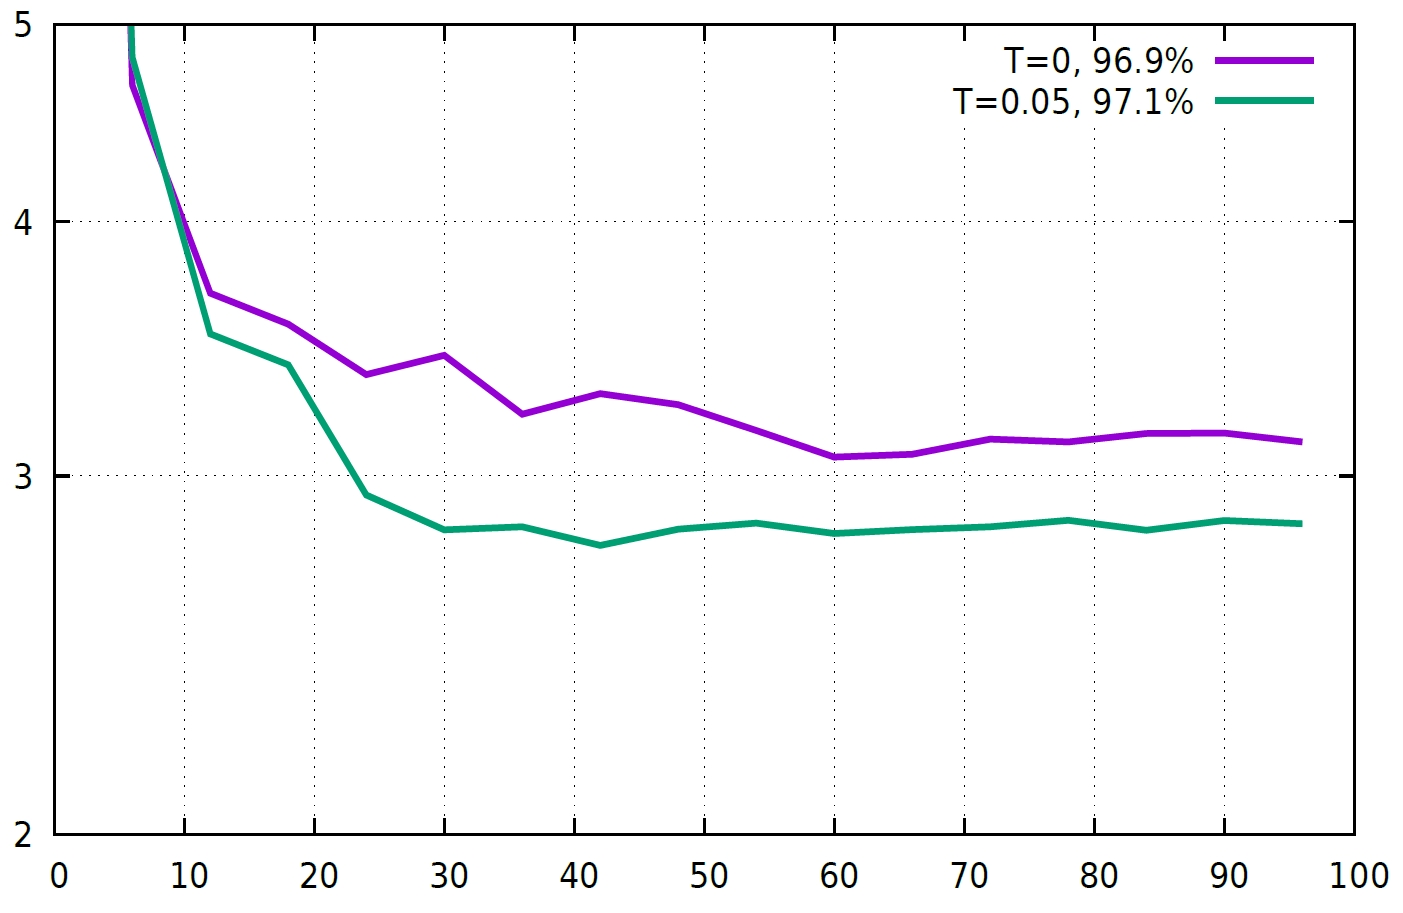
\includegraphics[width=.8\linewidth]{Imgs/mnist-.predicate-1png}\\
Error rate: DNNet - 3.1\%, \quad $\mathcal{VP}$-NNet - 2.9\%
\end{figure}
\end{frame}

\begin{frame}{EXAMPLE: MNIST DIGIT RECOGNITION}
Minimization of $R(f) = (Y - F(f))^{T}(\hat{\tau}V + \tau P)(Y - F(f))$.\\
2D image of digit $u_{i}(x^{1}, x^{2})$. 
\begin{center}
Predicate: $\phi(u_{i}) = \int_{0}^{1}\mathbf{u_{i}}(x^{1}, x^{2})\cos 2\pi x^{1}dx^{1}dx^{2}$.
\end{center}
Experiment settings: $\mathcal{V} = I, \ell = 1000$ (100 per class). Batch 6.
\begin{figure}
\centering
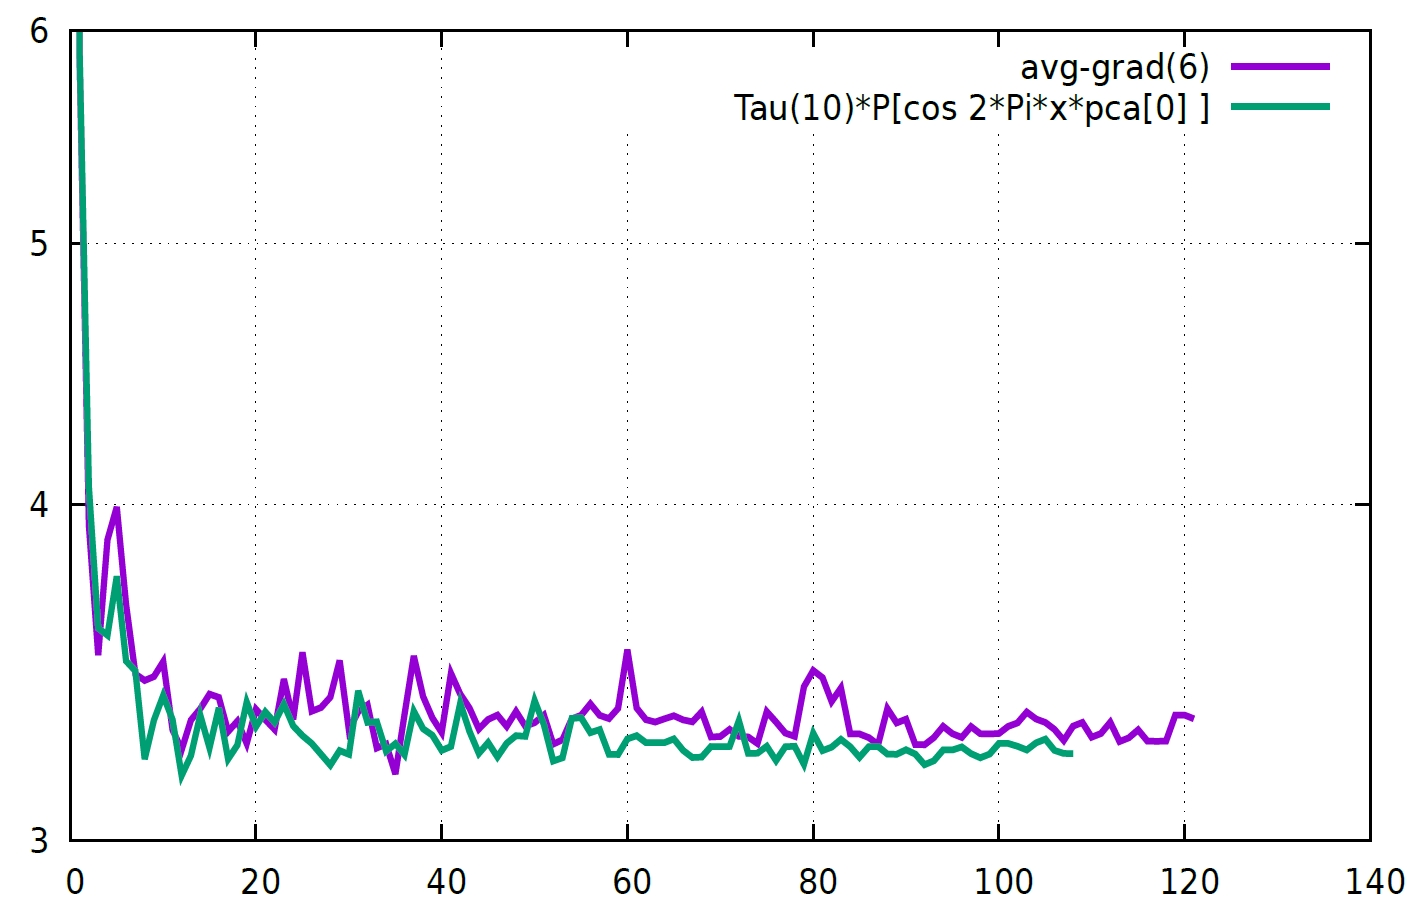
\includegraphics[width=.8\linewidth]{Imgs/mnist-.predicate-2png}\\
Error rate: DNNet - 3.4\%, \quad $\mathcal{VP}$-NNet - 3.3\%
\end{figure}
\end{frame}


\begin{frame}{EXAMPLE: MNIST DIGIT RECOGNITION}
Minimization of $R(f) = (Y - F(f))^{T}(\hat{\tau}V + \tau P)(Y - F(f))$.\\
\begin{center}
Predicate: $\phi(u_{i}) = \int_{0}^{1}\mathbf{u_{i}}(x^{1}, x^{2})\cos \mathbf{m}\pi x^{1}\cos \mathbf{n}\pi x^{2}dx^{1}dx^{2}$, m, n = 1, 2, 3, 4.
\end{center}
Experiment settings: $\mathcal{V} = I, \ell = 1000$ (100 per class). Batch 6.
\begin{figure}
\centering
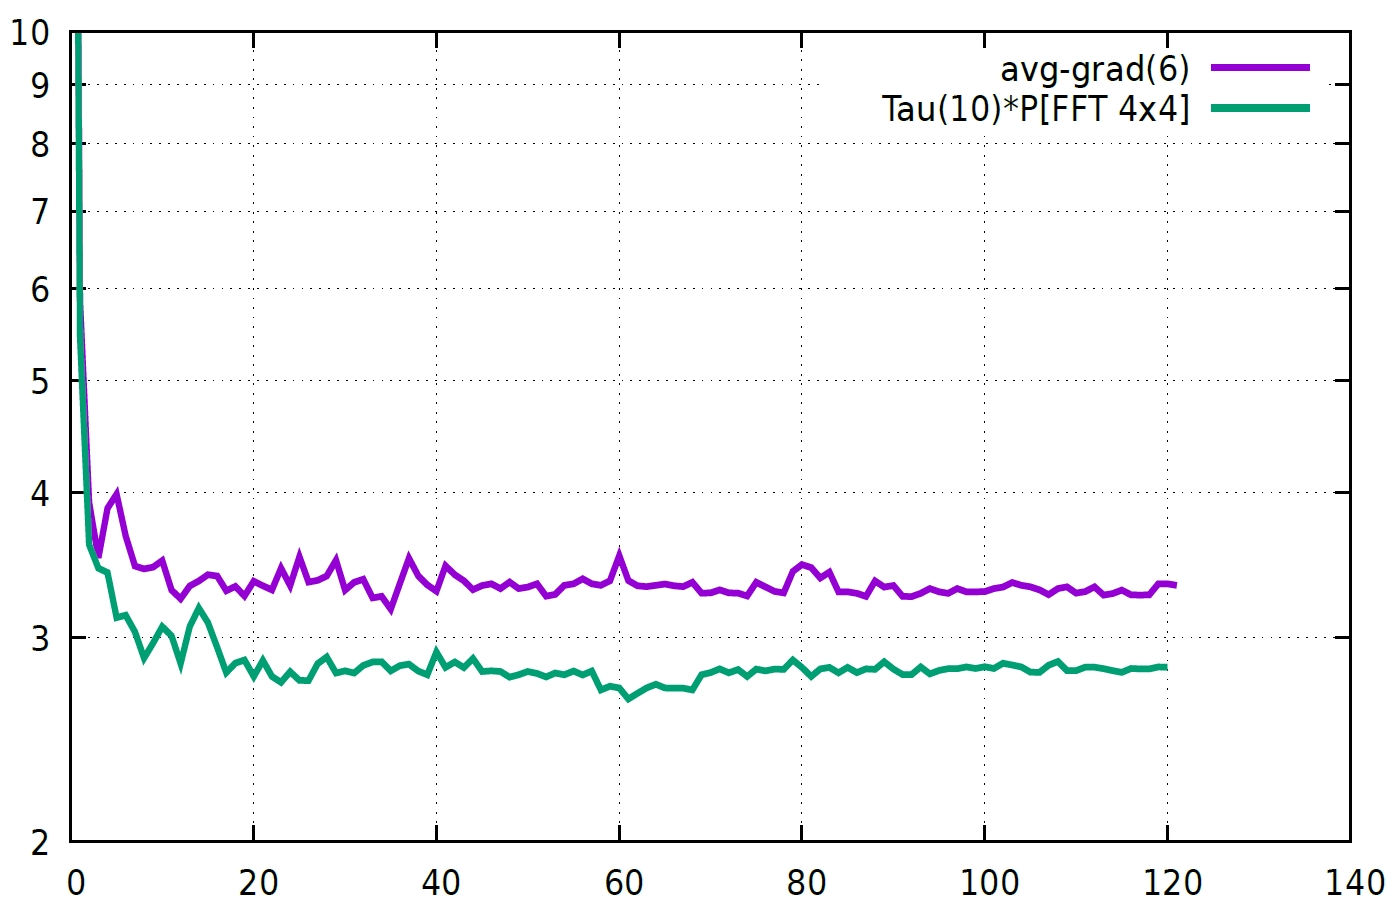
\includegraphics[width=.8\linewidth]{Imgs/mnist-.predicate-3png}\\
Error rate: DNNet - 3.4\%, \quad $\mathcal{VP}$-NNet - 2.8\%
\end{figure}
\end{frame}

\begin{frame}{STATISTICAL PART OF LEARNING THEORY IS COMPLETED}
\centering{Theory found that:}
\begin{enumerate}
\item The functional for minimization defines $\mathcal{V}$-quadratic form
\begin{align*}
R(f) = (Y - F(f))^{T}\mathcal{V}(Y - F(f)). \quad (1)
\end{align*}
\item In RKHS, where $F(f) = KA$, the admissible set of functions is defined by invariants for given $m$ predicates function $\phi_{k}$:
\begin{align*}
\Phi_{k}^{T}KA = \Phi_{k}^{T}Y, k = 1, \ldots, m. \quad (2)
\end{align*}
\item For RHKS the structure in SRM method is defined by the values of norm of functions from RKHS
\begin{align*}
A^{T}KA \leq C, \quad (3)
\end{align*}
which satisfies (2).
\item There exist unique (closed form) solution for the problem of minimization (1) subject to constraints (2) and (3).
\end{enumerate}
The only question left is "\emph{How to choose set of predicates}"? Answer to this question forms intelligent content of learning.
\end{frame}


\section{PART VI: EXAMPLES OF PREDICATES}
\begin{frame}
{\color{blue}{
\begin{center}
PART VI
\end{center}
\begin{center}
EXAMPLES OF PREDICATES
\end{center}
}}
\end{frame}


\begin{frame}{EXAMPLES OF GENERAL TYPE PREDICATES}
\begin{align*}
\sum_{i=1}^{\ell}P_{\ell}(y=1|x_{i})\phi(x_{i}) = \sum_{i=1}^{\ell}y_{i}\phi(x_{i}) \quad (*)
\end{align*}
\hrulefill
\begin{enumerate}
\item Predicate $\phi(x) = 1$ in (*) collects functions for which \emph{Expected number of elements of class $y=1$ computed using $P_{\ell}(y=1|x)$ equal to the number of training examples of the first class.}
\item Predicate $\phi(x) = x$ in (*) collects functions for which \emph{Expected center of mass of vectors $x$ of class $y=1$ computed using $P_{\ell}(y=1|x)$ coincides with center of mass of training examples of the first class.}
\item Predicate $\phi(x) = xx^{T}, x \in R^{n}$ collects functions for which \emph{Expected $0.5n(n + 1)$ values of covariance matrix computed using $P_{\ell}(y=1|x)$ coincide with values of covariance matrix computed for vectors $x$ of the first class.}
\end{enumerate}
\end{frame}

\begin{frame}{EXAMPLE OF PREDICATES FOR 2D IMAGES $\{u(x^{1}, x^{2})\}$}
Let $2D$ functions
\begin{align*}
u(x^{1}, x^{2}), 0 \leq x^{1}, x^{2} \leq \pi
\end{align*}
describe images and let $\ell$ pairs
\begin{align*}
(\mathbf{u_{1}}(x^{1}, x^{2}), y_{1}), \ldots, (\mathbf{u_{\ell}}(x^{1}, x^{2}), y_{\ell}),
\end{align*}
from the training set.
\begin{enumerate}
\item Predicates
\begin{align*}
\phi_{r, s}(\mathbf{u_{i}}) = \int_{0}^{\pi} \int_{0}^{\pi}\mathbf{u_{i}}(x^{1}, x^{2})\cos\mathbf{r}x^{1}\cos\mathbf{s}x^{2}dx^{1}dx^{2}, r, s = 1, \ldots, N
\end{align*}
define coefficients $a_{r, s}$ of cosines expansion of image $\mathbf{u_{i}}(x^{1}, x^{2})$.
\item For a given function $g(x^{1}, x^{2})$, predicate
\begin{align*}
\phi(\mathbf{u_{i}}, x_{\mu}, x_{\nu}) = \int_{-\infty}^{\infty}\int_{-\infty}^{\infty}\mathbf{u_{i}}(x^{1}, x^{2})g(x^{1} - x_{\mu}^{1}, x^{2} - x_{\nu}^{2})dx^{1}dx^{2},
\end{align*}
defines value of convolution at point $(x_{\mu}^{1}, x_{\nu}^{2})$.
\end{enumerate}
\end{frame}


\begin{frame}{INSTRUMENTS FOR SPECIAL PREDICATES}
\begin{center}
{\color{blue}{LIE DERIVATIVES}}
\end{center}
Let image is defined by differentiable 2D function $\mathbf{u}(x^{1}, x^{2})$. Consider small linear transformations of 2D space $(x^{1}, x^{2}) \in R^{2}$:
\begin{align*}
\mathbf{t}_\alpha\binom{x^1}{x^2} \Longrightarrow\binom{x^1+a_1 x^1+a_2 x^2+a_3}{x^2+a_4 x^2+a_5 x^1+a_6}
\end{align*}
For 	small $a_{k}$, function $\mathbf{u}(\mathbf{t}_{a}(x^{1}, x^{2}))$ in space $\mathbf{t}(x^{1}, x^{2})$ has the following representation in non-transformed space $(x^{1}, x^{2})$:
\begin{align*}
\mathbf{u}(\mathbf{t}_{\alpha}(x^{1}, x^{2})) \approx \mathbf{u}(x^{1}, x^{2}) + \sum_{k=1}^{6}\mathbf{a_{k}}\mathbf{L_{k}}\mathbf{u}(x^{1}, x^{2}),
\end{align*}
where $L_{k}\mathbf{u}(x^{1}, x^{2})$ are the so-called \textit{\textbf{Lie derivatives}}.
\footnote{Please make sense for the real meaning of this statements.}
\end{frame}

\begin{frame}{ILLUSTRATION}
Digit 2 in transformed space and 
\begin{figure}
\centering
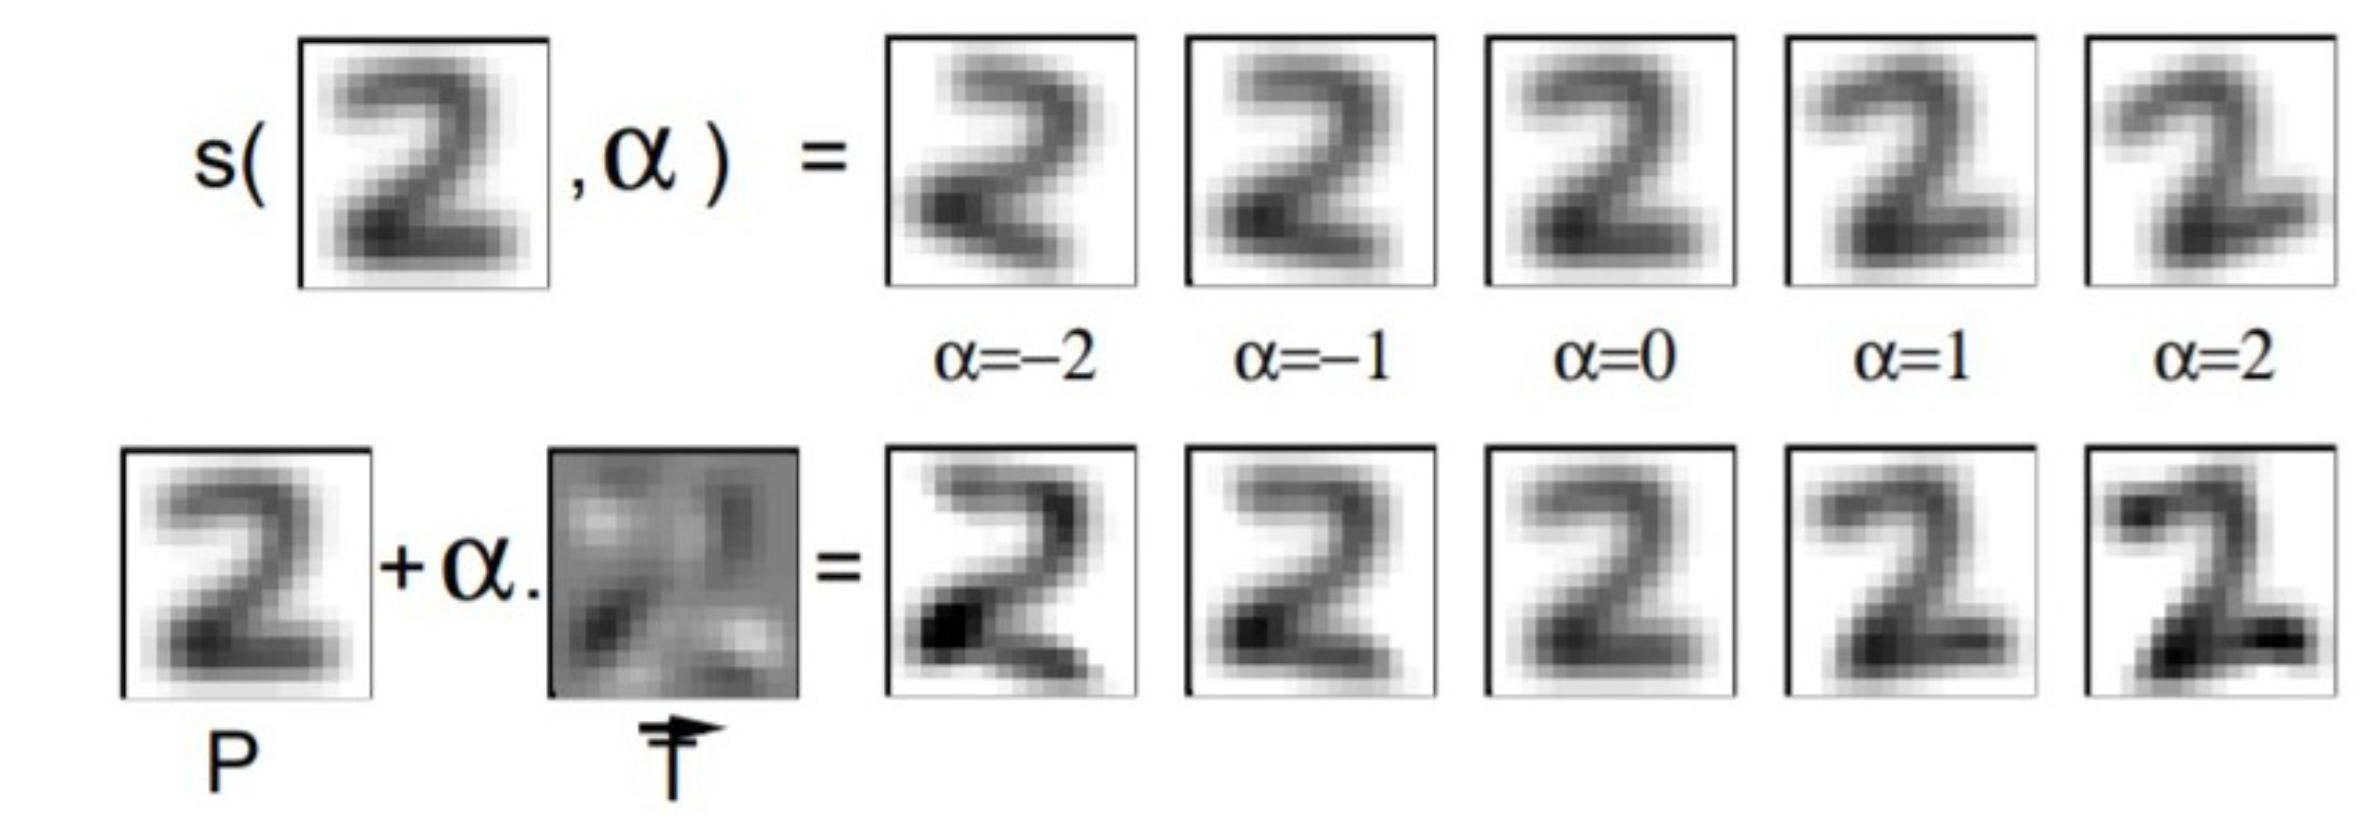
\includegraphics[width=1\linewidth]{Imgs/lie.png}\\
\end{figure}
\end{frame}


\begin{frame}{LIE OPERATIONS}

\end{frame}

\begin{frame}{ILLUSTRATION}

\end{frame}


\begin{frame}{INVARIANTS WITH RESPECT TO LINEAR TRANSFORMATIONS}

\end{frame}


\begin{frame}{TANGENT DISTANCE}

\end{frame}

\begin{frame}{EXAMPLES OF PREDICATES THAT DEFINE DEGREE OF SYMMETRIES}

\end{frame}

\begin{frame}{CONCLUSIVE REMARKS}
\begin{enumerate}
\item[•] Complete statistical methods of learning require, using structural risk minimization principle, in a given set of functions $\{f(x)\}$ minimize functional
\begin{align*}
R_{\mathcal{V}}(f) = (Y - F(f))^{T}\mathcal{V}(Y - F(f))
\end{align*}
subject to invariant constraints
\begin{align*}
\Phi_{s}^{T}F(f) = \Phi_{s}^{T}Y.
\end{align*}
\item[•] LUSI method provides unique solution of this problem for functions from RKHS and approximation for Neural Nets.
\item[•] Further progress in learning theory goes beyond statistical reasoning. It goes in the direction of search of predicates which form basis for understanding of problems existing in the World (see Plato-Hegel-Wigner line of philosophy).
\item[•] Predicates are abstract ideas, while invariants that are built using them from elements of solution. These two concepts reflect essence of intelligence, not just its imitation.
\end{enumerate}
\end{frame}

\begin{frame}{THE CHALLENGE}

\end{frame}


\begin{frame}{PLATO-HEGEL-WIGNER LINE OF PHILOSOPHY}
In 1928 Vladimir Propp published book "Morphology of the Folktale" where he described 31 predicates  that allow to synthesize Russian folk tales. Later his morphology has been successfully applied to other types of narrative, be it in \emph{literature, theater, film, television series, games, etc.} (although Propp applied it only to the wonder or fairy tale). (See Wikipedia: Vladimir Propp.) 

\hrulefill

The idea is that \emph{World of Ideas} contains small amount of ideas (predicates) that can be translated in \emph{Worlds of Things} by many different invariants.

\hrulefill

Propp found 31 predicates which describe different actions of people in Real World. Probably there exist a small amount of predicates that describe 2D \emph{Real World} images. The challenge is to find them (to understand \emph{World of 2D images}).
\end{frame}

\end{document}